\subsection{Canal de Comunicação}

\begin{questions}
\question{
Suponha o canal de comunicação discreto sem memória ilustrado na Figura \ref{fig:canal}.

   \begin{figure}[h!]
   \centering
   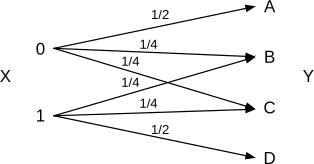
\includegraphics[width=0.3\textwidth]{../images/canal24.pdf}
   \caption{Canal de comunicação discreto sem memória.}
   \label{fig:canal}
   \end{figure}

\begin{parts}
\part Qual á a capacidade deste canal e qual é a distribuição em $X$ que alcança esta capacidade?

\part Assuma que $\Pr(X=0)=1/6$, $\Pr(X=1)=5/6$ e que a fonte não possui memória. Encontre o código ótimo
para comprimir a saída em $Y$. Qual é a comprimento médio das palavras do código? Calcule a entropia de $Y$ e compare com o comprimento médio encontrado para o código ótimo.

\end{parts}
}

\begin{solution}
\begin{parts}
\part 

Para este canal teremos a seguinte matriz de transmissão:

\begin{equation}
p(y|x) = 
\begin{pmatrix}
1/2 & 1/4 & 1/4 & 0   \\
0   & 1/4 & 1/4 & 1/2
\end{pmatrix}
\end{equation}

Podemos verificar que as linhas são permutação uma da outra
e a soma das colunas desta matriz é sempre $1/2$, logo trata-se 
de um canal simétrico fraco e assim poderemos calcular sua capacidade
através da equação
\begin{equation}
C = \log | \mathcal{Y} | - H(r)
\end{equation} 
onde $r$ é uma linha da matriz de transmissão.
Teremos assim
\begin{equation}
C = \log 4 - H\left( \frac{1}{2}, \frac{1}{4}, \frac{1}{4}, 0 \right) = 2 - \frac{3}{2} = \frac{1}{2} \text{ bit}.
\end{equation}

Como o canal é simétrico fraco, teremos que
\begin{align}
H(Y|X) &= \sum_x p(x) H(Y|X=x) \nonumber \\
       &= \sum_x p(x) H(r) \nonumber \\
       &= H(r)
\end{align}
e desta forma, não depende da distribuição da fonte $p(x)$. Para
encontrar a distribuição $p(x)$ que maximiza $I(X;Y)$, devemos então 
encontrar  $p(x)$ que maximiza $H(Y)$, pois teremos
\begin{align}
C &= \max_{p(x)} I(X;Y) \nonumber \\
  &= \max_{p(x)} H(Y) - H(Y|X) \nonumber \\
  &= \max_{p(x)} H(Y) - H(r) .
\end{align}
Como temos
\begin{align}
\Pr(Y=A) &= \frac{1}{2} p_0 \nonumber \\
\Pr(Y=B) &= \frac{1}{4} p_0 + \frac{1}{4} p_1 \nonumber \\
\Pr(Y=C) &= \frac{1}{4} p_0 + \frac{1}{4} p_1 \nonumber \\
\Pr(Y=D) &= \frac{1}{2} p_1 ,
\end{align}
$H(Y)$ será maximizado quando $p_0 = p_1 = 1/2$.

Utilizaremos aqui que
\begin{align}
C &= \max_{p(x)} I(X;Y) \nonumber \\
  &= \max_{p(x)} H(Y) - H(Y|X) .
\end{align}
Onde temos que
\begin{align}
H(Y|X) &= \sum_x p(x) H(Y|X=x) \nonumber \\
       &= p_0 H(Y|X=0) + p_1 H(Y|X=1) \nonumber \\
       &= p_0 H\left( \frac{1}{2} , \frac{1}{4}, \frac{1}{4} \right) + p_1 H\left( \frac{1}{4} , \frac{1}{4}, \frac{1}{2} \right) \nonumber \\
       &= \underbrace{(p_0 + p_1)}_{=1} H\left( \frac{1}{2} , \frac{1}{4}, \frac{1}{4} \right) \nonumber \\
       &= \frac{3}{2} .
\end{align}
Temos então que 
\begin{equation}
C = \max_{p(x)} H(Y) - \frac{3}{2} .
\end{equation}
Devemos agora analisar $H(Y)$, para tanto, usaremos $p(x)$ e $p(y|x)$.
\begin{align}
\Pr(Y=A) &= \frac{1}{2} p_0 \nonumber \\
\Pr(Y=B) &= \frac{1}{4} p_0 + \frac{1}{4} p_1 \nonumber \\
\Pr(Y=C) &= \frac{1}{4} p_0 + \frac{1}{4} p_1 \nonumber \\
\Pr(Y=D) &= \frac{1}{2} p_1 .
\end{align}
$H(Y)$ será maximizado quando $p_0 = p_1 = 1/2$, assim teremos
$H(Y) = H\left( \frac{1}{4} , \frac{1}{4}, \frac{1}{4}, \frac{1}{4} \right) = 2$ bits.
Logo, teremos
\begin{equation}
C = 2 - \frac{3}{2} = \frac{1}{2} \text{ bit}.
\end{equation}


\part 
Dada a distribuição em $X$, devemos calcular a distribuição em $Y$ para então
criar o código ótimo, um código de Huffman.
\begin{eqnarray}
\Pr(Y=A) &=& \frac{1}{2} p_0 = \frac{1}{12} \nonumber \\
\Pr(Y=B) &=& \frac{1}{4} p_0 + \frac{1}{4} p_1 = \frac{1}{4} \nonumber \\
\Pr(Y=C) &=& \frac{1}{4} p_0 + \frac{1}{4} p_1 = \frac{1}{4} \nonumber \\
\Pr(Y=D) &=& \frac{1}{2} p_1 = \frac{5}{12} 
\end{eqnarray}


\begin{minipage}[t]{0.6\textwidth}
\tikzset{every tree node/.style={align=left,anchor=north,minimum width=2em,draw,circle},
         blank/.style={draw=none},
         edge from parent/.style=
         {draw, edge from parent path={(\tikzparentnode) -- (\tikzchildnode)}},
         every node/.append style={align=left},
         level distance=1.5cm}
\begin{tikzpicture}[level distance=1.5cm,
  level 1/.style={sibling distance=5cm},
  level 2/.style={sibling distance=2.5cm},
  level 3/.style={sibling distance=2.5cm},
  level 4/.style={sibling distance=2.0cm},
  level 5/.style={sibling distance=1.5cm},
  % Skip a level in the tree
    skip level/.default={1},
    skip level/.style={
        level distance=\tikzleveldistance*#1+\tikzleveldistance},
    skip level spaced/.default={1},
    skip level spaced/.style={
        skip level=#1,
        sibling distance=\tikzsiblingdistance*#1+\tikzsiblingdistance},
  % code on edge:
    code/.style={
        insert path={edge from parent node[code label] {$#1$}}},
    code label/.style={outer sep=.5mm},
]
  \node {12/12}
  child { node {7/12} 
        child { node {4/12} 
                child { node {1/12 \\ A} [left, code=1] }
                child { node {3/12 \\ B} [right, code=0] }
                [left, code=1] 
        }
        child[skip level=1] { node {3/12 \\ C} [right, code=0] }
        [left, code=1] 
        }
  child[skip level=2] { node {5/12 \\ D} [right, code=0] }
;
\end{tikzpicture}
\end{minipage}
  \hfill
\begin{minipage}[c]{0.35\textwidth}
   %\vspace{-3em}
        % ($\sqcap$ e $\wedge$)
   \begin{center}
   \begin{tabular}[b]{clc}
        $x$ & $C(x)$ & $l(x)$ \\
        A & 111 & 3 \\
        B & 110 & 3 \\
        C & 10  & 2 \\
        D & 0   & 1 
   \end{tabular}
   \end{center}

   \ \\
   Comprimento esperado:
   \begin{eqnarray}
   L(C) &=& \sum_x p(y) l(y) = \nonumber \\
        &=& \frac{3}{12} + \frac{9}{12} + \frac{6}{12} + \frac{5}{12} \nonumber \\
        &\approx& 1.916  .
   \end{eqnarray}

   Entropia:
   \begin{align}
   H(Y) &= - \sum_y p(y) \log p(y) \nonumber \\ 
        &= \frac{1}{12} \log 12 + \frac{3}{12} \log 4 + \nonumber \\
         & \frac{1}{4} \log 4 + \frac{5}{12} \log \frac{12}{5} \nonumber \\
        &= 2 + \frac{1}{2} \log 3 - \frac{5}{12} \log 5 \nonumber \\
        &\approx 1.825 \text{ bits} .
   \end{align}

   Logo, temos $H(Y) \leq L(C)$, respeitando assim o teorema de Shannon.
\end{minipage}


\end{parts}
\end{solution}
\end{questions}
